\documentclass{article} % For LaTeX2e
\usepackage{iclr2016_conference,times}
\usepackage{hyperref}
\usepackage{url}
\usepackage{graphicx}
%\usepackage[outdir=./]{epstopdf}
\usepackage[cmex10]{amsmath}
\usepackage{array}
\usepackage{mdwmath}
\usepackage{mdwtab}
\usepackage{eqparbox}
\usepackage{tikz}
\usepackage{tikz-qtree}
\usepackage{stfloats}
\hyphenation{net-works Boltz-mann}
\usepackage{times}
\usepackage{xcolor}
\usepackage{amssymb}
\usepackage{epsfig}
\usepackage{amssymb}
\usepackage[]{algorithm2e}
\usepackage{floatrow}
% Table float box with bottom caption, box width adjusted to content
%\usepackage{capt-of}
%\usepackage[normalem]{ulem}
% \usepackage[all=normal,floats=tight,paragraphs=tight,indent=tight]{savetrees}
% \usepackage[subtle]{savetrees}

% \renewcommand{\baselinestretch}{0.97}

\newcommand{\argmax}{\arg\!\max}
\definecolor{green}{rgb}{0.2,0.8,0.2}
\definecolor{blue}{rgb}{0.2,0.2,0.8}
\usepackage{xspace}
\newcommand*{\eg}{e.g.\@\xspace}
\newcommand*{\ie}{i.e.\@\xspace}
\newcommand*{\aka}{a.k.a.\@\xspace}
\makeatletter
\newcommand*{\etc}{%
    \@ifnextchar{.}%
        {etc}%
        {etc.\@\xspace}%
}


\title{Sequence Level Training with\\Recurrent Neural Networks}


\author{Marc'Aurelio Ranzato, Sumit Chopra, Michael Auli, Wojciech Zaremba \\
Facebook AI Research\\
\texttt{\{ranzato, spchopra, michealauli, wojciech\}@fb.com}
}

% The \author macro works with any number of authors. There are two commands
% used to separate the names and addresses of multiple authors: \And and \AND.
%
% Using \And between authors leaves it to \LaTeX{} to determine where to break
% the lines. Using \AND forces a linebreak at that point. So, if \LaTeX{}
% puts 3 of 4 authors names on the first line, and the last on the second
% line, try using \AND instead of \And before the third author name.

\newcommand{\fix}{\marginpar{FIX}}
\newcommand{\new}{\marginpar{NEW}}
\newcommand{\bh}{\mathbf{h}}
\newcommand{\bb}{\mathbf{b}}
\newcommand{\bx}{\mathbf{x}}
\newcommand{\bc}{\mathbf{c}}
\newcommand{\bone}{\mathbf{1}}
\newcommand{\by}{\mathbf{y}}
\newcommand{\bs}{\mathbf{s}}
\newcommand{\btheta}{\mathbf{\theta}}
\newcommand{\bo}{\mathbf{o}}
\newcommand{\setr}{\mathcal{R}}
\newcommand{\mamark}[1]{\textcolor{orange}{{#1}}}
\newcommand{\spcmark}[1]{\textcolor{red}{{#1}}}
\newcommand{\macomment}[1]{\marginpar{\begin{center}\textcolor{orange}{#1}\end{center}}}
\iclrfinalcopy % Uncomment for camera-ready version



\begin{document}
\maketitle

%\baselinestretch{0.95}

\begin{abstract}
Many natural language processing applications use language models to generate text.
These models are typically trained to predict the next word in a sequence, given the previous words and some context such as an image. 
However, at test time the model is expected to generate the entire sequence from scratch. 
This discrepancy makes generation brittle, as errors may accumulate along the way. 
We address this issue by proposing a novel sequence level training algorithm that directly optimizes the metric used at test time, such as BLEU or ROUGE.
On three different tasks, our approach outperforms several strong baselines for greedy generation. The method is also competitive when these baselines employ beam search,
 while being several times faster. 
\end{abstract}

\section{Introduction}

Humans use different forms of communications such as speech, hand gestures and emotions. Being able to understand one's emotions and the encoded feelings is an important factor for an appropriate and correct understanding.


With the ongoing research in the field of robotics, especially in the field of humanoid robots, it becomes interesting to integrate these capabilities into machines allowing for a more diverse and natural way of communication. One example is the Software called EmotiChat~\cite{Anderson06areal-time}. This is a chat application with emotion recognition. The user is monitored and whenever an emotion is detected (smile, etc.), an emoticon is inserted into the chat window. Besides Human Computer Interaction other fields like surveillance or driver safety could also profit from it. Being able to detect the mood of the driver could help to detect the level of attention, so that automatic systems can adapt.\\
\let\thefootnote\relax\footnote{*F. Trier and P. Burkert contributed equally to this work.}


Many methods rely on extraction of the facial region. This can be realized through manual inference~\cite{4032815} or an automatic detection approach~\cite{Anderson06areal-time}.
Methods often involve the Facial Action Coding System (FACS) which describes the facial expression using Action Units (AU). An Action Unit is a facial action like "raising the Inner Brow". Multiple activations of AUs describe the facial expression~\cite{kumar2009face}. Being able to correctly detect AUs is a helpful step, since it allows making a statement about the activation level of the corresponding emotion. \\
Handcrafted facial landmarks can be used such as done by Kotsia et al.~\cite{4032815}. Detecting such landmarks can be hard, as the distance between them differs depending on the person~\cite{6998925}. Not only AUs can be used to detect emotions, but also texture. When a face shows an emotion the structure changes and different filters can be applied to detect this~\cite{6998925}.\\


\begin{figure}
   \centering
        \includegraphics[width=\columnwidth]{Fig1}
   \caption{Example images from the MMI (top) and CKP (bottom). The emotions from left to right are: \textit{Anger}, \textit{Sadness}, \textit{Disgust}, \textit{Happiness}, \textit{Fear}, \textit{Surprise}. The emotion \textit{Contempt} of the CKP set is not displayed.}\label{fig:example_images}
\end{figure}




The presented approach uses Artificial Neural Networks (ANN). ANNs differ, as they are trained on the data with less need for manual interference. 
Convolutional Neural Networks are a special kind of ANN and have been shown to work well as feature extractor when using images as input~\cite{donahue2013decaf} and are real-time capable. This allows for the usage of the raw input images without any pre- or postprocessing.\\
GoogleNet~\cite{DBLP:journals/corr/SzegedyLJSRAEVR14} is a deep neural network architecture that relies on CNNs. It has been introduced during the Image Net Large Scale Visual Recognition Challenge(ILSVRC) 2014. This challenge analyses the quality of different image classification approaches submitted by different groups. The images are separated into 1000 different classes organized by the WordNet hierarchy. In the challenge "object detection with additional training data" GoogleNet has achieved about 44\% precision~\cite{LSVRC-results}. These results have demonstrated the potential which lies in this kind of architecture. Therefore it has been used as inspiration for the proposed architecture.\\
The proposed network has been evaluated on the Extended Cohn-Kanade Dataset (Section~\ref{sec:ckp}) and on the MMI Dataset (Section~\ref{sec:mmi}). Typical pictures of persons showing emotions can be seen in Fig.~\ref{fig:example_images}.
The emotion \textit{Contempt} of the CKP set is not shown as no subject with consent for publication and an annotated emotion is part of the dataset. Results of experiments on these datasets demonstrate the success of using a deep layered neural network structure. With a 10-fold cross-validation a recognition accuracy of 99.6\% has been achieved. \\

The paper is arranged as follows: After this introduction, Related Work (Section~\ref{sec:related}) is presented which focuses on Emotion/Expression recognition and the various approaches scientists have taken. Next is Section~\ref{sec:background}, Background, which focuses on the main components of the architecture proposed in this article. Section~\ref{sec:datasets} contains a summary of the used Datasets. In Section~\ref{sec:architecture} the architecture is presented. This is followed by the experiments and its results (Section~\ref{sec:experiments}) . Finally, Section~\ref{sec:conclusion} summarizes the article and concludes the article.
\section{MT-DNN-1}
\label{sec:mt-dnn-1}

\subsection{Preliminaries}
\label{subsec:prelim}
In this work, our multi-task model combines classification, regression and pair-wise ranking tasks, which are summerised in Table~\ref{tab:task}. We briefly introduce the definition of each task as follows: 
\begin{table}[htb!]
	\begin{center}
		\begin{tabular}{@{\hskip1pt}l@{\hskip1pt}|@{\hskip1pt}c@{\hskip1pt}|@{\hskip1pt}c@{\hskip1pt}|@{\hskip1pt}c}
			\hline \bf Input &Classification&Regression &Ranking\\ \hline \hline
			single sentence &$\checkmark$&& \\
			pairwise text &$\checkmark$&$\checkmark$&$\checkmark$ \\ \hline
		\end{tabular}
	\end{center}
	\lgspace
	\caption{Summary of tasks in our multi-task framework.
	}
	\label{tab:task}
\lgspace
\end{table}
\begin{figure}[!t]
\centering
\adjustbox{trim={.065\width} {.01\height} {.05\width} {.01\height},clip}
{\includegraphics[scale=0.7]{mtl_model}}
\caption{Model architecture.}
\label{fig:mtl_model} 
\end{figure}

\begin{figure}[!t]
\centering
\adjustbox{trim={.05\width} {.01\height} {.05\width} {.01\height},clip}
{\includegraphics[scale=0.7]{mtl_model_v2}}
\caption{Model architecture version 2.}
\label{fig:mtl_model_v2} 
\end{figure}

\textbf{Task definition}

\textbf{Objective}

\textbf{Single classification}
\xiaodl{Need to cluster different tasks..}

\textbf{Sentence-pair classification}: given a pair of sentence, $(S_1, S_2)$, the model predicts a label indicating the relation of this pair of sentences: $P(C|S_1, S_2)$. For example, natural language inference is a typical instance of the sentence-pair classification task: a premise and a hypothesis are denoted by $S_1$ and $S_2$, respectively; the label, $C$, belongs one of three relations (\textit{contradiction}, \textit{neutral} and \textit{entailment}). 

\textbf{Regression}


\textbf{Pair-wise Ranking}
\begin{algorithm}[ht!]
 \SetAlgoLined
Initialize model parameters $\Theta$ randomly  \\
Set M \quad\textit{//the number of updates for the shared layer} \\
%\textit{Counter} = 0\\
 \For{$iteration$ in $0 ... \infty$}{
 	 %1. \textit{Counter} += 1\\
     1. Pick a task $t$ randomly \\
     2. Pick sample(s) from task $t$, i.e., \\
     \hspace{0.4cm}$(Q,C=\{0,1\})$ for classification \\
     \hspace{0.4cm}$(Q, D)$ for ranking\\
     3. Compute loss: $L(\Theta)$, i.e.,\\
     \hspace{0.4cm} the \textit{cross-entropy} for classification \\
     \hspace{0.4cm} the ranking loss for ranking\cite{learning-to-rank2005burges}\\

     4. Compute gradient: $\nabla(\Theta)$ \\
     5. Update model: $\Theta = \Theta - \epsilon \nabla(\Theta)$ \quad\textit{}
     % \eIf{Counter $<$ M}{
  	 %5. Update model: $\Theta = \Theta - \epsilon \nabla(\Theta)$ \quad\textit{//update both $\Theta^s$ and $\Theta^t$} \\
   %}{
   	% 6. Update model: $\Theta^t = \Theta^t - \epsilon \nabla(\Theta^t)$ 
  %}
 }
 \caption{\label{algo:mtdnn} Training a Multi-task model.}
 \algorithmfootnote{Note that $\Theta$ denotes the model parameters. \textcolor{red}{TODO: update alg based on task defination.}}
\end{algorithm}
% !TEX root = ../multi_task.tex

We evaluate the presented MTL method on a number of problems. First, we use MultiMNIST \citep{multi_mnist}, an MTL adaptation of MNIST \citep{mnist}. Next, we tackle multi-label classification on the CelebA dataset \citep{celeba} by considering each label as a distinct binary classification task. These problems include both classification and regression, with the number of tasks ranging from 2 to 40. Finally, we experiment with scene understanding, jointly tackling the tasks of semantic segmentation, instance segmentation, and depth estimation on the Cityscapes dataset \citep{cityscapes}. We discuss each experiment separately in the following subsections.

The baselines we consider are (i) \textbf{uniform scaling:} minimizing a uniformly weighted sum of loss functions \mbox{$\frac{1}{T}\sum_t \lL^t$}, \mbox{(ii) \textbf{single task:}} solving tasks independently, \mbox{(iii) \textbf{grid search:}} exhaustively trying various values from $\{ c^t \in [0,1] | \sum_t c^t = 1\}$ and optimizing for $\frac{1}{T}\sum_t c^t \lL^t$, \mbox{(iv) \textbf{\citet{Kendall2018}:}} using the uncertainty weighting proposed by \citet{Kendall2018}, and \mbox{(v) \textbf{GradNorm:}} using the normalization proposed by \citet{Chen2018}.



\subsection{MultiMNIST}
\label{sec:multi_mnist_exp}

Our initial experiments are on MultiMNIST, an MTL version of the MNIST dataset \citep{multi_mnist}. In order to convert digit classification into a multi-task problem, \citet{multi_mnist} overlaid multiple images together. We use a similar construction. For each image, a different one is chosen uniformly in random. Then one of these images is put at the top-left and the other one is at the bottom-right. The resulting tasks are: classifying the digit on the top-left (task-L) and classifying the digit on the bottom-right (task-R). We use 60K examples and directly apply existing single-task MNIST models. The MultiMNIST dataset is illustrated in the supplement.

We use the LeNet architecture \citep{mnist}. We treat all layers except the last as the representation function $g$ and put two fully-connected layers as task-specific functions (see the supplement for details). We visualize the performance profile as a scatter plot of accuracies on task-L and task-R in Figure~\ref{fig:multi_mnist_performance_curve}, and list the results in Table~\ref{tab:multi_mnist}.

In this setup, any static scaling results in lower accuracy than solving each task separately (the single-task baseline). The two tasks appear to compete for model capacity, since increase in the accuracy of one task results in decrease in the accuracy of the other. Uncertainty weighting \citep{Kendall2018} and GradNorm \citep{Chen2018} find solutions that are slightly better than grid search but distinctly worse than the single-task baseline. In contrast, our method finds a solution that efficiently utilizes the model capacity and yields accuracies that are as good as the single-task solutions. This experiment demonstrates the effectiveness of our method as well as the necessity of treating MTL as multi-objective optimization. Even after a large hyper-parameter search, \emph{any} scaling of tasks does not approach the effectiveness of our method.



\subsection{Multi-Label Classification}

\begin{figure}[t]
\includegraphics[width=\textwidth]{radar_full_new}
\vspace{1mm}
\caption{Radar charts of percentage error per attribute on CelebA \citep{celeba}. Lower is better. We divide attributes into two sets for legibility: easy on the left, hard on the right. Zoom in for details.}
\label{fig:multi_label_radar}
\end{figure}


\begin{wraptable}{r}{0.3\textwidth}
%\vspace{-4mm}
\captionof{table}{Mean of error per category of MTL algorithms in multi-label classification on CelebA \citep{celeba}.}
\begin{tabular}{r@{\hspace{2mm}}c@{}}
\toprule
& Average  \\
&  error \\
\midrule
Single task & $8.77$ \\
Uniform scaling & $9.62$ \\
\citealt{Kendall2018} & $9.53$ \\
GradNorm & $8.44$ \\
Ours & $\mathbf{8.25}$  \\
\bottomrule
\end{tabular}
\label{table:multi_label_bar}
%\vspace{-5mm}
\end{wraptable}

Next, we tackle multi-label classification. Given a set of attributes, multi-label classification calls for deciding whether each attribute holds for the input. We use the CelebA dataset \citep{celeba}, which includes 200K face images annotated with 40 attributes. Each attribute gives rise to a binary classification task and we cast this as a 40-way MTL problem. We use ResNet-18 \citep{resnet} without the final layer as a shared representation function, and attach a linear layer for each attribute (see the supplement for further details).


We plot the resulting error for each binary classification task as a radar chart in Figure~\ref{fig:multi_label_radar}. The average over them is listed in Table~\ref{table:multi_label_bar}. We skip grid search since it is not feasible over 40 tasks. Although uniform scaling is the norm in the multi-label classification literature, single-task performance is significantly better. Our method outperforms baselines for significant majority of tasks and achieves comparable performance in rest. This experiment also shows that our method remains effective when the number of tasks is high.


\subsection{Scene Understanding}

To evaluate our method in a more realistic setting, we use scene understanding. Given an RGB image, we solve three tasks: semantic segmentation (assigning pixel-level class labels), instance segmentation (assigning pixel-level instance labels), and monocular depth estimation (estimating continuous disparity per pixel). We follow the experimental procedure of \citet{Kendall2018} and use an encoder-decoder architecture. The encoder is based on ResNet-50 \citep{resnet} and is shared by all three tasks. The decoders are task-specific and are based on the pyramid pooling module \citep{pspnet} (see the supplement for further implementation details).

Since the output space of instance segmentation is unconstrained (the number of instances is not known in advance), we use a proxy problem as in \citet{Kendall2018}. For each pixel, we estimate the location of the center of mass of the instance that encompasses the pixel. These center votes can then be clustered to extract the instances. In our experiments, we directly report the MSE in the proxy task. Figure~\ref{fig:cityscapes_performance_profile} shows the performance profile for each pair of tasks, although we perform all experiments on all three tasks jointly. The pairwise performance profiles shown in Figure~\ref{fig:cityscapes_performance_profile} are simply 2D projections of the three-dimensional profile, presented this way for legibility. The results are also listed in Table~\ref{tab:cityscapes_results}.

MTL outperforms single-task accuracy, indicating that the tasks cooperate and help each other. Our method outperforms all baselines on all tasks.


\subsection{Role of the Approximation}

In order to understand the role of the approximation proposed in Section~\ref{sec:approximation}, we compare the final performance and training time of our algorithm with and without the presented approximation in Table~\ref{tab:approximation_tradeoff} (runtime measured on a single Titan Xp GPU). For a small number of tasks (3 for scene understanding), training time is reduced by 40\%. For the multi-label classification experiment (40 tasks), the presented approximation accelerates learning by a factor of 25.

On the accuracy side, we expect both methods to perform similarly as long as the full-rank assumption is satisfied. As expected, the accuracy of both methods is very similar. Somewhat surprisingly, our approximation results in slightly improved accuracy in all experiments. While counter-intuitive at first, we hypothesize that this is related to the use of SGD in the learning algorithm. Stability analysis in convex optimization suggests that if gradients are computed with an error $\hat{\nabla}_\btheta \mathcal{L}^t = \nabla_\btheta \mathcal{L}^t + \mathbf{e}^t$ ($\btheta$ corresponds to $\btheta^{sh}$ in (\ref{eq:kkt_opt})), as opposed to $\mathbf{Z}$ in the approximate problem in \ref{eq:approx}, the error in the solution is bounded as $\|\hat{\mathbf{\alpha}} - \mathbf{\alpha} \|_2 \leq \mathcal{O}(\max_t \|\mathbf{e}^t\|_2)$. Considering the fact that the gradients are computed over the full parameter set (millions of dimensions) for the original problem and over a smaller space for the approximation (batch size times representation which is in the thousands), the dimension of the error vector is significantly higher in the original problem. We expect the $l_2$ norm of such a random vector to depend on the dimension.

In summary, our quantitative analysis of the approximation suggests that (i) the approximation does not cause an accuracy drop and (ii) by solving an equivalent problem in a lower-dimensional space, our method achieves both better computational efficiency and higher stability.

  {\small
  \begin{table}[t]
%  \vspace{-4mm}
  \caption{Effect of the MGDA-UB approximation. We report the final accuracies as well as training times for our method with and without the approximation.}
  %\vspace{1mm}
  \centering
  \begin{tabular}{@{}r@{\hspace{3mm}}c@{\hspace{3mm}}c@{\hspace{2mm}}c@{\hspace{2mm}}c@{}c@{\hspace{5mm}}c@{\hspace{2mm}}c@{}}
  \toprule
  & \multicolumn{4}{c}{Scene understanding (3 tasks)} &  & \multicolumn{2}{c}{Multi-label (40 tasks)}  \\
  \cmidrule(r){2-5} \cmidrule(lr){7-8}
                  & Training & Segmentation & Instance  & Disparity      & & Training & Average \\
                 & time     &  mIoU [\%]       & error [px] & error [px] & & time (hour)      & error \\
  \midrule
  Ours (w/o approx.) & $38.6$ & $66.13$ & $10.28$ & $2.59$ & & $429.9$ & $8.33$ \\
  Ours & $\mathbf{23.3}$ & $\mathbf{66.63}$ & $\mathbf{10.25}$ & $\mathbf{2.54}$  & & $\mathbf{16.1}$ & $\mathbf{8.25}$ \\
  \bottomrule
  \end{tabular}
  %\vspace{-2mm}
  \label{tab:approximation_tradeoff}
  \end{table}}

\section{Conclusions}

Our work is motivated by two major deficiencies in training the current generative models for text generation: exposure bias and a loss which does not operate at the sequence level.
While Reinforcement learning can potentially address these issues, it struggles in settings when 
there are very large action spaces, such as in text generation. Towards that end, 
we propose the MIXER algorithm, which deals with these issues and enables successful training of reinforcement learning models for text generation. 
We achieve this by replacing the initial random policy with the optimal policy of a cross-entropy trained model and by gradually exposing the model more and more to its own predictions in an incremental learning framework.




%. First, the exposure bias affecting the commonly used cross-entropy loss. 
%While the model sees only ground truth inputs at training time, at test time model predictions are fed back as input to generate a full sequence. 
%Second, current text generation systems are often trained to predict the next word in the sequence without taking into account the quality of the % overall sequence. 
% These discrepancies make the generation process brittle.
%Reinforcement learning is a framework that can address these issues. 
%First, at training time the model is used to generate an entire sequence of actions. 
%Second, the reward does not need to factor over individual words nor does it need to be differentiable. 
%Therefore, we can easily and directly operate at the sequence level, generate at training time and optimize our model towards any desired metric, such as BLEU and ROUGE. 
%One challenge with reinforcement learning is that it struggles with very large action spaces such as for text generation.

% Mixed Incremental Cross-Entropy Reinforce (MIXER) 
%The algorithm we propose, MIXER, 
%deals with this issue and enables successful training of reinforcement learning models for text generation. 
%We achieve this by replacing the initial random policy with the optimal policy of a cross-entropy trained model and by gradually exposing the model more and more to its own predictions in an incremental learning framework.

Our results show that MIXER outperforms three strong baselines for greedy generation and it is very competitive with beam search. 
The approach we propose is agnostic to the underlying model or the form of the reward function. 
% We are free to use any other metric as reward such as ROUGE or METEOR instead of BLEU. 
% Similarly, we may use a different parametric model such as a feed- forward network or an LSTM \citep{lstm}.
In future work we would like to design better estimation techniques for the average reward $\bar{r}_t$, because poor estimates can lead to slow convergence of both REINFORCE and MIXER. 
Finally, our training algorithm relies on a single sample while it would be interesting to investigate the effect of more comprehensive search methods at training time.


% Our work addresses two major deficiencies in training the current generative models for text generation. First, it addresses the {\it exposure bias} affecting the commonly used cross-entropy loss. 
% %While the model sees only ground truth inputs at training 
% %time, at test time model predictions are fed back as input to generate a full sequence. 
% Second, it directly tries to optimize for the final evaluation metric, namely, BLEU. 
% %current text generation systems are often trained to predict the next word in the sequence without taking into account the quality of the overall sequence. These discrepancies make the generation process brittle. 
% Both these objectives are accomplished by the proposed Mixed Incremental Cross-Entropy Reinforce (MIXER) algorithm. 
% %Reinforcement learning is a framework that can address these issues. First, at training time the model is used to generate an entire sequence of actions. Second, the reward does not need to factor over individual words nor does it need to be differentiable. Therefore, we can easily and directly operate at the sequence level, generate at training time and optimize our model towards BLEU, our test time evaluation metric. One challenge with reinforcement learning is that it struggles with very large action spaces such as for text generation.
% MIXER is an extension of the REINFORCE algorithm applied to text generation, which 
% %Mixed Incremental Cross-Entropy Reinforce (MIXER) deals with this issue and enables
% %successful training of reinforcement learning models for text generation.
% replaces the initial random policy with the optimal policy of
% a cross-entropy trained model and it gradually exposes the model more and more to its own predictions in an incremental learning framework.

% Our results show that MIXER outperforms three strong baselines for greedy generation and it is very competitive with beam search. 
% The approach we propose is agnostic to the underlying model or the form of the reward function. 
% We are free to use any other metric as reward such as ROUGE or METEOR instead of BLEU. 
% Similarly, we may use a different parametric model such as a feed-forward network or an LSTM~\citep{lstm}.

% For future we would like to design better estimation techniques for the average reward $\bar{r}_t$, because poor estimates can lead to slow convergence of both REINFORCE and MIXER.
% Finally, our training algorithm relies on a single sample while it would be interesting to investigate the effect of more comprehensive search methods at training time.

% In this study, we investigated sequence level training algorithms for RNNs with the goal to improve text generation.
% Today, the dominant training protocol is cross-entropy loss, which optimizes the prediction of the next word in the sequence. However, at test time the model is asked to predict several words in the future by re-circulating its own prediction back to the input. 
% The problem of predicting several steps in the future while obtaining delayed feedback, and to perform prediction via a discrete sequence of actions inspired us to apply reinforcement learning techniques. Unfortunately, reinforcement learning techniques do not usually handle well large action spaces, like those we encounter in typical language modeling applications.

% MIXER addresses these limitations through pre-training and incremental learning. 

% MIXER addresses these limitations by leveraging both the fact that we have access to the optimal policy and by using incremental learning.
% Since we have examples of ground truth generation, we can "pre-train" the model for next step prediction via cross-entropy. This drastically reduces the actual search space. By using incremental learning, the model is then able to gradually produce stable sequences and to make effective use of its own predictions.

% Our empirical validation shows that the model we propose achieves the best BLEU score compared to three strong baselines. Moreover, generations can be further improved by using beam search. Note that the approach we proposed is agnostic of the particular underlying model and metric. We can easily replace BLEU with ROUGE, METEOR, \etc by simply swapping the function that computes rewards within the training loop. Similarly, the training algorithm applies to any type of model and RNN, LSTM~\citep{lstm} included.



% There are several avenues of future investigation. First, REINFORCE upon which we build, requires careful estimation of the average reward. Poor estimation of this value can yield very slow convergence. More generally, searching at training time is still an unsolved problem. In particular, it would be very powerful to include beam search also at training time. 


\subsubsection*{Acknowledgments}
The authors would like to thank David Grangier, Tomas Mikolov, Leon Bottou, Ronan Collobert and Laurens van der Maaten for their insightful comments. 
We also would like to thank Alexander M. Rush for his help in preparing the data set for the summarization task and Sam Gross for providing the image features. 

\bibliography{iclr2016_conference}
\bibliographystyle{iclr2016_conference}
\newpage
\section{Supplementary Material}


\subsection{Experiments}


\subsubsection{Qualitative Comparison}
\begin{figure}[h!]
\tiny{
\begin{verbatim}


CONTEXT:      a chinese government official on sunday dismissed reports that the government was delaying the issuing
              of third generation -lrb- #g -rrb- mobile phone licenses in order to give a developing <unk> system an
              advantage
GROUND TRUTH: foreign phone operators to get equal access to china 's #g market
XENT:         china dismisses report of #g mobile phone phone
DAD:          china denies <unk> <unk> mobile phone licenses
E2E:          china 's mobile phone licenses delayed
MIXER:        china official dismisses reports of #g mobile licenses

CONTEXT:      greece risks bankruptcy if it does not take radical extra measures to fix its finances , prime minister
              george papandreou warned on tuesday , saying the country was in a `` wartime situation
GROUND TRUTH: greece risks bankruptcy without radical action
XENT:         greece warns <unk> measures to <unk> finances
DAD:          greece says no measures to <unk> <unk>
E2E:          greece threatens to <unk> measures to <unk> finances
MIXER:        greece does not take radical measures to <unk> deficit

CONTEXT:      the indonesian police were close to identify the body parts resulted from the deadly explosion in front
              of the australian embassy by the dna test , police chief general <unk> <unk> said on wednesday
GROUND TRUTH: indonesian police close to <unk> australian embassy bomber
XENT:         indonesian police close to <unk>
DAD:          indonesian police close to <unk>
E2E:          indonesian police close to monitor deadly australia
MIXER:        indonesian police close to <unk> parts of australian embassy

CONTEXT:      hundreds of catholic and protestant youths attacked security forces with <unk> bombs in a flashpoint
              area of north belfast late thursday as violence erupted for the second night in a row , police said
GROUND TRUTH: second night of violence erupts in north belfast
XENT:         urgent hundreds of catholic and <unk> <unk> in <unk>
DAD:          hundreds of belfast <unk> <unk> in n. belfast
E2E:          hundreds of catholic protestant , <unk> clash with <unk>
MIXER:        hundreds of catholic <unk> attacked in north belfast

CONTEXT:      uganda 's lord 's resistance army -lrb- lra -rrb- rebel leader joseph <unk> is planning to join his
              commanders in the ceasefire area ahead of talks with the government , ugandan army has said
GROUND TRUTH: rebel leader to move to ceasefire area         
XENT:         uganda 's <unk> rebel leader to join ceasefire
DAD:          ugandan rebel leader to join ceasefire talks
E2E:          ugandan rebels <unk> rebel leader
MIXER:        ugandan rebels to join ceasefire in <unk>

CONTEXT:      a russian veterinary official reported a fourth outbreak of dead domestic poultry in a suburban
              moscow district sunday as experts tightened <unk> following confirmation of the presence of the 
              deadly h#n# bird flu strain
GROUND TRUTH: tests confirm h#n# bird flu strain in # <unk> moscow <unk>
XENT:         russian official reports fourth flu in <unk>
DAD:          bird flu outbreak in central china
E2E:          russian official official says outbreak outbreak outbreak in <unk>
MIXER:        russian official reports fourth bird flu

CONTEXT:      a jewish human rights group announced monday that it will offer <unk> a dlrs ##,### reward for 
              information that helps them track down those suspected of participating in nazi atrocities during 
              world war ii
GROUND TRUTH: jewish human rights group offers reward for information on nazi suspects in lithuania
XENT:         jewish rights group announces <unk> to reward for war during world war
DAD:          rights group announces <unk> dlrs dlrs dlrs reward
E2E:          jewish rights group offers reward for <unk>
MIXER:        jewish human rights group to offer reward for <unk>

CONTEXT:      a senior u.s. envoy reassured australia 's opposition labor party on saturday that no decision 
              had been made to take military action against iraq and so no military assistance had been sought 
              from australia
GROUND TRUTH: u.s. envoy meets opposition labor party to discuss iraq
XENT:         australian opposition party makes progress on military action against iraq
DAD:          australian opposition party says no military action against iraq
E2E:          us envoy says no decision to take australia 's labor
MIXER:        u.s. envoy says no decision to military action against iraq

CONTEXT:      republican u.s. presidential candidate rudy giuliani met privately wednesday with iraqi president 
              jalal talabani and indicated that he would keep a u.s. presence in iraq for as long as necessary , 
              campaign aides said
GROUND TRUTH: giuliani meets with iraqi president , discusses war
XENT:         <unk> meets with president of iraqi president
DAD:          republican presidential candidate meets iraqi president
E2E:          u.s. president meets with iraqi president
MIXER:        u.s. presidential candidate giuliani meets with iraqi president
\end{verbatim}
}
\caption{Examples of greedy generations after conditioning on sentences from the test summarization dataset. The "$<$unk$>$" token is produced by our tokenizer and it replaces rare words.} 
\label{fig:generation}
\end{figure}


\subsubsection{Hyperparameters}
\begin{table}[!h]
\caption{Best scheduling parameters found by hyper-parameter search of MIXER.}
\begin{tabular}{l || l | l | l}
      \multicolumn{1}{c||}{\emph{TASK} }  & 
      \multicolumn{1}{c|}{$N^{\mbox{\small XENT}}$} & 
      \multicolumn{1}{c|}{$N^{\mbox{\small XE+R}}$} & \multicolumn{1}{c}{$\Delta$} \\
      \hline
      \hline
      {\em summarization} & 20 & 5 & 2  \\
      \hline
      {\em machine translation} & 25 & 5 & 3 \\
      \hline
      {\em image captioning} & 20 & 5 & 2  \\
    \end{tabular}
\label{tab:scheduling}
\end{table}

\subsubsection{Relative Gains}


\begin{figure}[!h]
\begin{center}
 \includegraphics[width=0.6\linewidth]{summarization_bleu_rouge.pdf}
 \end{center}
\caption{Relative gains on summarization with respect to the XENT baseline. Left: relative BLEU score. Right: relative ROUGE-2.
The models are: DAD, E2E, MIXER trained for the objective used at test time (method proposed in this paper), and MIXER trained with a different metric.
When evaluating for BLEU, the last column on the left reports the evaluation of MIXER trained using ROUGE-2.
When evaluating for ROUGE-2, the last column on the right reports the evaluation of MIXER trained using BLEU.}
\label{fig:summarization_bleu_rouge}
\end{figure}



\vspace{0.3in}
\begin{figure}[!h]
  \centering
  \begin{minipage}{0.05\linewidth}
  	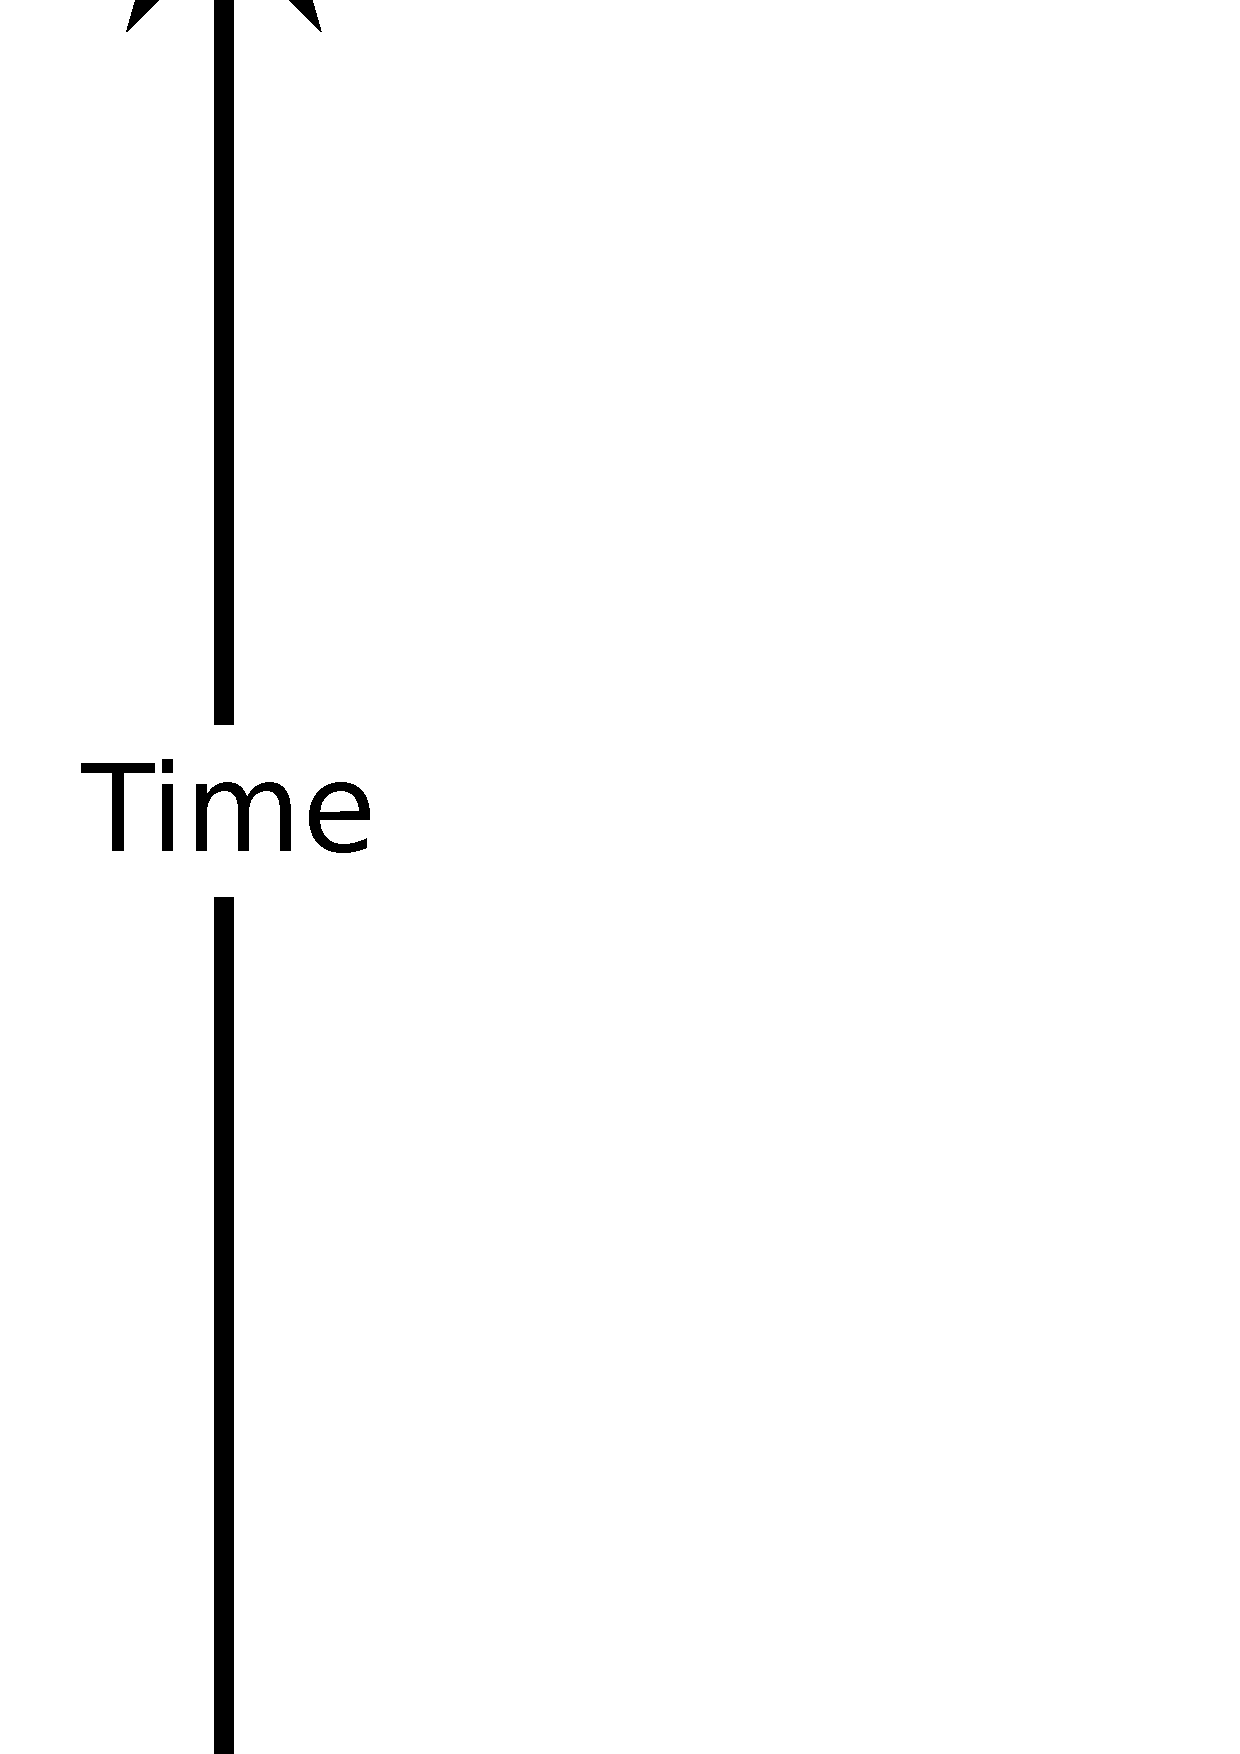
\includegraphics[width=2.5\linewidth]{time.pdf}\\
  \end{minipage}
  \begin{minipage}{0.46\linewidth}
  	\centering
    \scalebox{0.75}{
    \tiny
    \begingroup\makeatletter\def\f@size{1}\check@mathfonts
    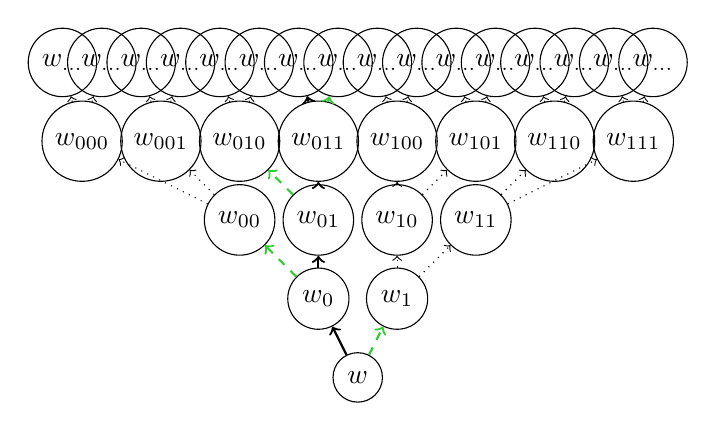
\begin{tikzpicture}
      \node [draw, circle] (w) at (0,0) {$w$};
      \node [draw, circle] (w0) at (-0.5,1) {$w_0$};
      \node [draw, circle] (w1) at (0.5,1) {$w_1$};
      \node [draw, circle] (w00) at (-1.5,2) {$w_{00}$};
      \node [draw, circle] (w01) at (-0.5,2) {$w_{01}$};
      \node [draw, circle] (w10) at (0.5,2) {$w_{10}$};
      \node [draw, circle] (w11) at (1.5,2) {$w_{11}$};
      \node [draw, circle] (w000) at (-3.5,3) {$w_{000}$};
      \node [draw, circle] (w001) at (-2.5,3) {$w_{001}$};
      \node [draw, circle] (w010) at (-1.5,3) {$w_{010}$};
      \node [draw, circle] (w011) at (-0.5,3) {$w_{011}$};
      \node [draw, circle] (w100) at (0.5,3) {$w_{100}$};
      \node [draw, circle] (w101) at (1.5,3) {$w_{101}$};
      \node [draw, circle] (w110) at (2.5,3) {$w_{110}$};
      \node [draw, circle] (w111) at (3.5,3) {$w_{111}$};
      \node [draw, circle] (w0000) at (-3.75,4) {$w_{\dots}$};
      \node [draw, circle] (w0001) at (-3.25,4) {$w_{\dots}$};
      \node [draw, circle] (w0010) at (-2.75,4) {$w_{\dots}$};
      \node [draw, circle] (w0011) at (-2.25,4) {$w_{\dots}$};
      \node [draw, circle] (w0100) at (-1.75,4) {$w_{\dots}$};
      \node [draw, circle] (w0101) at (-1.25,4) {$w_{\dots}$};
      \node [draw, circle] (w0110) at (-0.75,4) {$w_{\dots}$};
      \node [draw, circle] (w0111) at (-0.25,4) {$w_{\dots}$};
      \node [draw, circle] (w1000) at (0.25,4) {$w_{\dots}$};
      \node [draw, circle] (w1001) at (0.75,4) {$w_{\dots}$};
      \node [draw, circle] (w1010) at (1.25,4) {$w_{\dots}$};
      \node [draw, circle] (w1011) at (1.75,4) {$w_{\dots}$};
      \node [draw, circle] (w1100) at (2.25,4) {$w_{\dots}$};
      \node [draw, circle] (w1101) at (2.75,4) {$w_{\dots}$};
      \node [draw, circle] (w1110) at (3.25,4) {$w_{\dots}$};
      \node [draw, circle] (w1111) at (3.75,4) {$w_{\dots}$};
      \draw [thick] [->] (w) to (w0);
      \draw [thick] [dashed] [green] [->] (w) to (w1);
      \draw [thick] [dashed] [green] [->] (w0) to (w00);
      \draw [thick] [->] (w0) to (w01);
      \draw [dotted] [->] (w1) to (w10);
      \draw [dotted] [->] (w1) to (w11);
      \draw [dotted] [->] (w00) to (w000);
      \draw [dotted] [->] (w00) to (w001);
      \draw [thick] [dashed] [green] [->] (w01) to (w010);
      \draw [thick] [->] (w01) to (w011);
      \draw [dotted] [->] (w10) to (w100);
      \draw [dotted] [->] (w10) to (w101);
      \draw [dotted] [->] (w11) to (w110);
      \draw [dotted] [->] (w11) to (w111);
      \draw [dotted] [->] (w000) to (w0000);
      \draw [dotted] [->] (w000) to (w0001);
      \draw [dotted] [->] (w001) to (w0010);
      \draw [dotted] [->] (w001) to (w0011);
      \draw [dotted] [->] (w010) to (w0100);
      \draw [dotted] [->] (w010) to (w0101);
      \draw [thick] [->] (w011) to (w0110);
      \draw [thick] [dashed] [green] [->] (w011) to (w0111);
      \draw [dotted] [->] (w100) to (w1000);
      \draw [dotted] [->] (w100) to (w1001);
      \draw [dotted] [->] (w101) to (w1010);
      \draw [dotted] [->] (w101) to (w1011);
      \draw [dotted] [->] (w110) to (w1100);
      \draw [dotted] [->] (w110) to (w1101);
      \draw [dotted] [->] (w111) to (w1110);
      \draw [dotted] [->] (w111) to (w1111);
      \end{tikzpicture}
      \endgroup
    }\\
    Training with exposure bias
  \end{minipage}
  \begin{minipage}{0.46\linewidth}
  	\centering
    \scalebox{0.75}{
    \tiny
    \begingroup\makeatletter\def\f@size{1}\check@mathfonts
    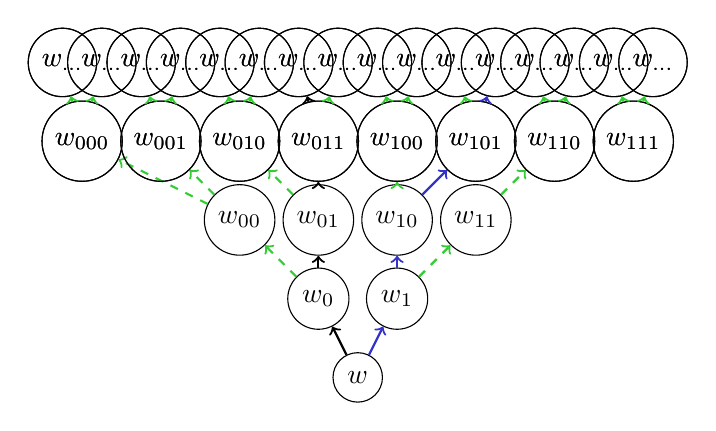
\begin{tikzpicture}
      \node [draw, circle] (w) at (0,0) {$w$};
      \node [draw, circle] (w0) at (-0.5,1) {$w_0$};
      \node [draw, circle] (w1) at (0.5,1) {$w_1$};
      \node [draw, circle] (w00) at (-1.5,2) {$w_{00}$};
      \node [draw, circle] (w01) at (-0.5,2) {$w_{01}$};
      \node [draw, circle] (w10) at (0.5,2) {$w_{10}$};
      \node [draw, circle] (w11) at (1.5,2) {$w_{11}$};
      \node [draw, circle] (w000) at (-3.5,3) {$w_{000}$};
      \node [draw, circle] (w001) at (-2.5,3) {$w_{001}$};
      \node [draw, circle] (w010) at (-1.5,3) {$w_{010}$};
      \node [draw, circle] (w011) at (-0.5,3) {$w_{011}$};
      \node [draw, circle] (w100) at (0.5,3) {$w_{100}$};
      \node [draw, circle] (w101) at (1.5,3) {$w_{101}$};
      \node [draw, circle] (w110) at (2.5,3) {$w_{110}$};
      \node [draw, circle] (w111) at (3.5,3) {$w_{111}$};
      \node [draw, circle] (w0000) at (-3.75,4) {$w_{\dots}$};
      \node [draw, circle] (w0001) at (-3.25,4) {$w_{\dots}$};
      \node [draw, circle] (w0010) at (-2.75,4) {$w_{\dots}$};
      \node [draw, circle] (w0011) at (-2.25,4) {$w_{\dots}$};
      \node [draw, circle] (w0100) at (-1.75,4) {$w_{\dots}$};
      \node [draw, circle] (w0101) at (-1.25,4) {$w_{\dots}$};
      \node [draw, circle] (w0110) at (-0.75,4) {$w_{\dots}$};
      \node [draw, circle] (w0111) at (-0.25,4) {$w_{\dots}$};
      \node [draw, circle] (w1000) at (0.25,4) {$w_{\dots}$};
      \node [draw, circle] (w1001) at (0.75,4) {$w_{\dots}$};
      \node [draw, circle] (w1010) at (1.25,4) {$w_{\dots}$};
      \node [draw, circle] (w1011) at (1.75,4) {$w_{\dots}$};
      \node [draw, circle] (w1100) at (2.25,4) {$w_{\dots}$};
      \node [draw, circle] (w1101) at (2.75,4) {$w_{\dots}$};
      \node [draw, circle] (w1110) at (3.25,4) {$w_{\dots}$};
      \node [draw, circle] (w1111) at (3.75,4) {$w_{\dots}$};

      \draw [thick] [->] (w) to (w0);
      \draw [thick] [blue] [->] (w) to (w1);
      \draw [thick] [dashed] [green] [->] (w0) to (w00);
      \draw [thick] [->] (w0) to (w01);
      \draw [thick] [blue] [->] (w1) to (w10);
      \draw [thick] [dashed] [green] [->] (w1) to (w11);
      \draw [thick] [dashed] [green] [->] (w00) to (w000);
      \draw [thick] [dashed] [green] [->] (w00) to (w001);
      \draw [thick] [dashed] [green] [->] (w01) to (w010);
      \draw [thick] [->] (w01) to (w011);
      \draw [thick] [dashed] [green] [->] (w10) to (w100);
      \draw [thick] [blue] [->] (w10) to (w101);
      \draw [thick] [dashed] [green] [->] (w11) to (w110);
      \node [draw, circle] (w000) at (-3.5,3) {$w_{000}$};
      \node [draw, circle] (w001) at (-2.5,3) {$w_{001}$};
      \node [draw, circle] (w010) at (-1.5,3) {$w_{010}$};
      \node [draw, circle] (w011) at (-0.5,3) {$w_{011}$};
      \node [draw, circle] (w100) at (0.5,3) {$w_{100}$};
      \node [draw, circle] (w101) at (1.5,3) {$w_{101}$};
      \node [draw, circle] (w110) at (2.5,3) {$w_{110}$};
      \node [draw, circle] (w111) at (3.5,3) {$w_{111}$};
      \node [draw, circle] (w0000) at (-3.75,4) {$w_{\dots}$};
      \node [draw, circle] (w0001) at (-3.25,4) {$w_{\dots}$};
      \node [draw, circle] (w0010) at (-2.75,4) {$w_{\dots}$};
      \node [draw, circle] (w0011) at (-2.25,4) {$w_{\dots}$};
      \node [draw, circle] (w0100) at (-1.75,4) {$w_{\dots}$};
      \node [draw, circle] (w0101) at (-1.25,4) {$w_{\dots}$};
      \node [draw, circle] (w0110) at (-0.75,4) {$w_{\dots}$};
      \node [draw, circle] (w0111) at (-0.25,4) {$w_{\dots}$};
      \node [draw, circle] (w1000) at (0.25,4) {$w_{\dots}$};
      \node [draw, circle] (w1001) at (0.75,4) {$w_{\dots}$};
      \node [draw, circle] (w1010) at (1.25,4) {$w_{\dots}$};
      \node [draw, circle] (w1011) at (1.75,4) {$w_{\dots}$};
      \node [draw, circle] (w1100) at (2.25,4) {$w_{\dots}$};
      \node [draw, circle] (w1101) at (2.75,4) {$w_{\dots}$};
      \node [draw, circle] (w1110) at (3.25,4) {$w_{\dots}$};
      \node [draw, circle] (w1111) at (3.75,4) {$w_{\dots}$};
      \draw [thick] [dashed] [green] [->] (w000) to (w0000);
      \draw [thick] [dashed] [green] [->] (w000) to (w0001);
      \draw [thick] [dashed] [green] [->] (w001) to (w0010);
      \draw [thick] [dashed] [green] [->] (w001) to (w0011);
      \draw [thick] [dashed] [green] [->] (w010) to (w0100);
      \draw [thick] [dashed] [green] [->] (w010) to (w0101);
      \draw [thick] [->] (w011) to (w0110);
      \draw [thick] [dashed] [green] [->] (w011) to (w0111);
      \draw [thick] [dashed] [green] [->] (w100) to (w1000);
      \draw [thick] [dashed] [green] [->] (w100) to (w1001);
      \draw [thick] [dashed] [green] [->] (w101) to (w1010);
      \draw [thick] [blue] [->] (w101) to (w1011);
      \draw [thick] [dashed] [green] [->] (w110) to (w1100);
      \draw [thick] [dashed] [green] [->] (w110) to (w1101);
      \draw [thick] [dashed] [green] [->] (w111) to (w1110);
      \draw [thick] [dashed] [green] [->] (w111) to (w1111);
      \end{tikzpicture}
      \endgroup
    }
	Training in expectation (Reinforce)
  \end{minipage}
  \caption{Search space for the toy case of a binary vocabulary and sequences of length 4.  
    The trees represent all the $2^4$ possible sequences.
  The solid black line is the ground truth sequence. 
  \textbf{(Left)} Greedy training such as XENT optimizes only the probability 
  of the next word. The model may consider choices indicated by the green arrows, but it starts off from words taken from the ground truth sequence. The model experiences exposure bias, since it sees only words branching off the ground truth path;
  \textbf{(Right)} REINFORCE and MIXER optimize over all possible sequences, using the predictions made by the model itself.  
  In practice, the model samples only a single path indicated by the blue solid line. The model does not suffer from exposure bias; the model is trained as it is tested.}
  \label{fig:plan}
\end{figure}

  


    


\subsection{The Attentive Encoder}
\label{sup-material:encoder}
Here we explain in detail how we generate the conditioning vector $\bc_t$ 
for our RNN using the source sentence and the current hidden state $\bh_t$. 
Let us denote by $\bs$ the source sentence which is composed of a sequence 
of $M$ words $\bs = [w_1, \ldots, w_M]$. 
With a slight overload of notation let $w_i$ also denote the $d$ dimensional 
learnable embedding of the $i$-th word ($w_i \in \setr^d$). In addition the 
position $i$ of the word $w_i$ is also associated with a learnable embedding $l_i$ 
of size $d$ ($l_i \in \setr^d$). Then the full embedding for 
the $i$-th word in the input sentence is given by $a_i = w_i + l_i$. 
In order for the embeddings to capture local context, we associate an 
aggregate embedding $z_i$ to each word in the source sentence. 
In particular for a word in the $i$-th position, its aggregate embedding 
$z_i$ is computed by taking a window of $q$ consecutive words centered 
at position $i$ and averaging the embeddings of all the words in this window. More precisely, the aggregate embedding $z_i$ is given by: 
\begin{equation}
z_i = \frac{1}{q} \sum_{h = -q/2}^{q/2} a_{i + h}. 
\end{equation}
In our experiments the width $q$ was set to $5$. 
In order to account for the words at the two boundaries of the input 
sentence we first pad the sequence on both sides with dummy words before 
computing the aggregate vectors $z_i$s. Given these aggregate vectors of words, we compute 
the context vector $c_t$ (the final output of the encoder) as: 
\begin{equation}
c_t = \sum_{j=1}^M \alpha_{j,t} w_j, 
\end{equation}
where the weights $\alpha_{j, t}$ are computed as 
\begin{equation}
\alpha_{j, t} = \frac{\exp(z_j \cdot \bh_{t})}{\sum_{i=1}^M \exp(z_i \cdot \bh_{t})}.
\end{equation}



\subsection{Beam Search Algorithm}
\label{sup-material:beam_search}
Equation~\ref{eq:greedy_gen} always chooses the highest scoring next word candidate
at each time step. At test time we can reduce the effect of search error 
by pursuing not only one but $k$ next word candidates at each point, which 
is commonly known as {\it beam search}.
While still approximate, this strategy can recover higher scoring sequences 
that are often also better in terms of our final evaluation metric.
The algorithm maintains the $k$ highest scoring partial
sequences, where $k$ is a hyper-parameter.
Setting $k=1$ reduces the algorithm to a greedy left-to-right search 
(Eq.~\eqref{eq:greedy_gen}). 
%The downside of such an exploration of multiple paths is that it significantly slows down the generation process. The time complexity 
%grows linearly in $k$ because we need to perform $k$ forward passes for our network which is the most time intensive operation. 
%As a result, beam search generation is $k$ times slower than greedy search (Eq.~\eqref{eq:greedy_gen}). 
\begin{algorithm}[!h]
  \KwIn{model $p_{\theta}$, beam size $k$}
  \KwResult{sequence of words $[w_1^g, w_2^g, \dots, w_n^g]$}
  empty heaps $\{\mathcal{H}_t\}_{t = 1, \dots T}$\;
  an empty hidden state vector $\bh_1$\;
  $\mathcal{H}_1.\mbox{push}(1, [[\varnothing], \bh_1])$\;
  \For{$t\leftarrow 1$ \KwTo $T - 1$}{	
    \For{$i\leftarrow 1$ \KwTo $\min(k, \#\mathcal{H}_t)$}{
      $(p, [[w_1, w_2, \dots, w_t], \bh]) \leftarrow \mathcal{H}_t.\mbox{pop}()$\;  
      $\bh' = \phi_\theta(w, \bh)$ \;      
      \For{$w' \leftarrow$ $k$-most likely words $w'$ from $p_\theta(w' | w_t, \bh)$}{
        $p' = p * p_\theta(w' | w, \bh)$\;
        $\mathcal{H}_{t + 1}.\mbox{push}(p', [[w_1, w_2, \dots, w_t, w'], \bh'])$\;
      }
    }
  }
  $(p, [[w_1, w_2, \dots, w_T], \bh]) \leftarrow \mathcal{H}_T.\mbox{pop}()$\;
  \KwOut{$[w_1, w_2, \dots, w_T]$}
 
 \caption{Pseudo-code of beam search with beam size $k$.}
  \label{alg:beam} 
\end{algorithm}


\newpage






\subsection{Notes}
The current version of the paper updates the first version uploaded on arXiv as follows:
\begin{itemize}
\item on the summarization task, we report results using both ROUGE-2 and BLEU to demonstrate that MIXER can work with any metric.
\item on machine translation and image captioning we use LSTM instead of Elman RNN to demonstrate the MIXER can work with any underlying parametric model.
\item BLEU is evaluated using up to 4-grams, and it is computed at the corpus level (except in the image captioning case) as this seems the most common practice
in the summarization and machine translation literature.
\item we have added several references as suggested by our reviewers
\item we have shortened the paper by moving some content to the Supplementary Material. 
\end{itemize}

\end{document}